\documentclass[12pt]{article}
\usepackage{graphicx}
%\usepackage{showframe}
\usepackage[top=1.0in, bottom=1.0in, left=1.5in, right=1.0in]{geometry}
\title{A Modern Version Of Space Invaders}
\author{Rian Fitzgerald}
\parindent 0ex
\setlength{\parskip}{1em}

\usepackage{listings}
\usepackage{color}
\definecolor{dkgreen}{rgb}{0,0.6,0}
\definecolor{gray}{rgb}{0.5,0.5,0.5}
\definecolor{mauve}{rgb}{0.58,0,0.82}


\begin{document}
\pagenumbering{gobble}
%\maketitle
\newpage

\begin{center}
\section*{}
	
\includegraphics[scale=1]{uni-limerick-crest.png}
	
	{\Large Department of Computer Science and Information Systems
	
	\vspace{5em}
	Title: A modern version of Space Invaders
	
	By: Rian Fitzgerald 13121626
	
	Course: Computer Games Development LM110
	
	Supervisor: Annette McElligott}
	
\end{center}
\newpage
\pagenumbering{roman}
\section*{Project Summary}
This project is an advanced version of the classic game Space Invaders. It will retain some of the core mechanics and add some features that will provide a challenge for the player. 

There are two parts to this project, the game and the supporting website. The website is used to create accounts for players as well as having a leader board which displays data about the player (for example, their high score, time played and highest level achieved). 

This project uses the same perspective as the original game (top down, two dimensional). The difference between this version and the original is that it is more difficult to beat as the player's score increases. The objective of the game is to survive as long as possible while achieving the highest score possible. 

This project uses modern tools and techniques as this was a limiting factor in the original implementation. These factors are discussed in more detail in the Background and Research portion of this report. 

The technologies used in this project are the Unity game engine, NodeJS, MongoDB and AngularJS. The game retains how the player and enemies move on the screen and the scoring mechanics (when an enemy dies, their value is added to the players score). The features that include the enemies becoming harder to defeat as the player's score increases and the information being passed to a server. 

\newpage
\section*{Acknowledgments}
I would like to acknowledge my family and friends for providing guidance and support for me during my years at college. 
\newpage
\section*{Declaration}
This final year project is presented in partial fulfilment of the requirement for the Bachelor of Science in Computer Games Development. I herewith declare that I have produced this report without prohibited assistance of third parties and without making use of aids others than those specified. Where use has been made of the work of other people if has been fully acknowledged and referenced appropriately. 

Signature: \underline{\hspace{5cm}}

Date: \underline{\hspace{5.9cm}}
\newpage

\begin{center}
\tableofcontents
\end{center}

\newpage
\pagenumbering{arabic}

\section{Introduction}


\subsection{General Introduction}
This chapter will give a brief description of the chapters that follow. Chapter 2  discusses that background and research that went into this project. Chapter 3 will showcase some of the design that went into this project. Chapter 4 will address some of the implementation and issues encountered. Chapter 5 will showcase the testing and evaluation used in the project. The final chapter discusses the conclusions and possible further development of this project.

\subsection{Motivating Factors}
The main motivation for undertaking this project was to improve the Space Invaders game. From the research completed (of Chapter 3), many clones have a set difficulty. This results in an imbalance in the difficulty. A highly skilled player will be able to get a high score quite easily. The result of this project has created a game that will make it more difficult a player to beat. 

A secondary motivation to complete this project was to become familiar with using a modern game engine. It would be a useful skill to add to my repertoire, especially if I want to apply for a job in a game company after college. 

Another motivation for doing this project is to increase my knowledge in web based technologies. As most companies have a web presence it would be useful to know about web technologies, especially those based around JavaScript. 

The final motivation for completing this project is to combine the knowledge I have learned from various modules. This project incorporates aspects of Programming, Object Orientated Programming, Database Systems, Distributed Systems and Systems Analysis and Design. Principles learned from these modules will be applied in the project

\subsection{Objectives of Proposed Work}
This project has two key objectives with multiple elements to be completed. The two primary objectives are the game and the website. 

The following list details the objectives to be completed for the game.

\begin{enumerate}
\item Programming the initial game using simple graphics.
\item Refining the game mechanics.
\item Program a login screen for the game to allow a player to login so their details can
be recorded.
\end{enumerate}

The following list details the objectives to be completed for the website.

\begin{enumerate}
\item Programming the website.
\item Programming the server.
\item Responding to any GET, POST, PUT and DELETE commands to make the
website RESTful.
\item Creating the database and populating it with test data.
\item Use a testing framework to test if the correct data is being transferred to the
various parts of the project.
\end{enumerate}
\newpage

\section{Background and Research}
The background and research section discusses the previous implementations of Space Invaders and the considerations that the original designer had to consider. It will also analyse the technologies that will power this project. 

\subsection{Analysis of Existing Products}
The original Space Invaders was very primitive in its implementation. It was so primitive that it was unable to render many colours and had to rely on a colour overlay (arcade-museum.com, 2016). The specification for some of the system is:


\begin{itemize}
	\item Processor: Intel 8080
	\item Raster graphics on a CRT monitor
	\item Texas Instruments SN76477
\end{itemize}

An interesting point to note is that the graphics were drawn using the processor. This was due to the lack of dedicated graphics processing units at the time. It also explains why the graphics were primitive by today's standards (for example, pixel based with little colouring).

In 1980 a version of Space Invaders was ported to the Atari 2600 (gamespy.com, 2016). This had a number of advantages over the original. The biggest advantage was that the colour palette was increased. Other hardware improvements included the addition of RAM and cartridges that could have memory included (problemkaputt.de/, 2016).

At the time of writing this report, there are many clones that exist. These clones are available on many platforms from the original game to iOS (kotaku.com, 2016). These clones can differ in many ways from the original. Some will have different aesthetics while others will have different mechanics. Table 1 shows a compiled list of some of the data available about clones of Space Invaders (bandainamcoent.eu, gamespy.com, ign.com, kotaku.com, theisozone.com, 2017).

\begin{center}
    \begin{tabular}{ | p{3cm} | p{2.5cm} | p{2cm} | p{4cm} |} \hline
    Name & Platform(s) & Released & Features \\ \hline
    Space Invaders (Original) & Arcade, Atari 2600, Nintendo Entertainment System, iOS & 1978, 1980, 1985, 2009 & Raster graphics \\ \hline
    
    Space Invaders Part II, Space Invaders Deluxe (USA) & Arcade, Game Boy & 1979, 1990 & Gameboy version allowed multiplayer, USA version had updated graphics\\ \hline
    
    Space Invaders '95 & Arcade & 1995 & Updated graphics  \\ \hline
    
	Space Invaders 1999, Space Invaders X (Japan) & Playstation, PC, Nintendo 64, Game Boy Color & 1999 & 2D and 3D graphics, competitive mode, cooperative mode,   \\ \hline 
	
	Space Invaders Evolution, Space Invaders: Galaxy Beat (Japan) & Playstation Portable & 2005 & Updated graphics, sounds and gameplay, multiplayer mode, rhythm action gameplay \\ \hline
	
	Space Invaders Extreme & Nintendo DS, Playstation Portable, Xbox 360 & 2008, 2009 & Integrated musical elements \\ \hline
	
	Space Invaders Infinity Gene & iOS, Playstation 3, Xbox 360, Android & 2009, 2010, 2013 & Updated graphics\\ \hline
    \end{tabular}
\end{center}

\begin{center}
Table 1
\end{center}

\newpage
\subsection{Unity Game Engine}
The Unity engine is a multiplatform game engine. It allows developers to target a range of devices for example PC, Android, iOS and Xbox, to name a few. It uses one click deployment to build solutions for as many devices that are required (https://unity3d.com/, 2016).

The engine supports a multitude of file formats for images, audio, video and text. The engine abstracts the more difficult aspects of creating a game such as optimisation and graphics rendering. For graphics, it targets APIs depending on which system is selected for the build. Windows can use both Direct3D and OpenGL, Android and iOS use OpenGL ES and consoles use proprietary APIs.

Programming in Unity can be achieved by using a number of languages. The most widely used language for Unity is C{\#}. JavaScript can also be used; however, it is not the same JavaScript that is used for web browsers. It is commonly referred to as UnityScript (answers.unity3d.com/, 2016). A third language called Boo was also available, however it is now deprecated. It is not documented by Unity anymore, although it will still compile (forum.unity3d.com, 2016).

Due to its better support and documentation, C{\#} will be the language used to implement the game portion of this project.

\subsection{Unreal Engine}
Another popular choice for developing games is Unreal Engine. It is one of the biggest competitors to Unity. It is also a multiplatform game engine and can export builds for a range of devices such as PC, Mac, Linux, Xbox and Playstation, to name a few (https://www.unrealengine.com).

As with Unity, Unreal Engine supports many file formats. It also enables developers to accomplish more as the more difficult parts of game programming is abstracted. Programming in Unreal is achieved using two methods. The first is using C++ and utilising the Unreal API. The second method uses Blueprints. Blueprints in Unreal are a style of visual coding where the developer drags, drops and connects nodes to get the desired functionality. However these Blueprints are not as good performance wise when compared to C++ (https://forums.unrealengine.com, 2017). 

\subsection{MongoDB}
MongoDB is a high performance, scalable, document orientated NoSQL database solution. (stackoverflow.com, 2017). MongoDB uses a JSON-like document with schemas. JSON is a lightweight data format that is easy for humans to read and write as well as to parse for machines. Figure 1 shows an example of some data in the JSON format.

JSON is built upon two structures: 
\begin{itemize}
	\item A collection of key/value pairs that correspond to an abject, record, dictionary, hash table, keyed list or an associative array, depending on which language is being used.
	\item A list of ordered values that correspond to an array, vector or similar data structure. (json.org, 2017)
\end{itemize}

\begin{center}
	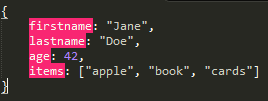
\includegraphics[scale=1]{json_no_id.PNG}

	Figure 1: Data in JSON format
\end{center}

Because MongoDB is a NoSQL solution the schema is not enforced as strictly as it would in a relational database. The dynamic schema means that each document can have different key/value pairs and can still be inserted into the database. Table 2 shown below summarises the differences between a Relational Database Management System (for example, MySQL) and MongoDB.

\begin{center}
    \begin{tabular}{| l | l |}
    \hline
    \textbf{Relational Database Management System} & \textbf{MongoDB}  \\ \hline
    Table & Collection \\ \hline
    Tuple or Row & Document \\ \hline
    Column & Field \\ \hline
    Primary Key & Key id provided by MongoDB \\ \hline
    \end{tabular}
\end{center}

\begin{center}
Table 2
\end{center}

The {\_}id provided by MongoDB is a 12 byte hexadecimal number which ensures the uniqueness of each document. This hexadecimal number is construced as follows:

\begin{itemize}
	\item The first 4 bytes are a timestamp since the ObjectId's creation. This uses the seconds elapsed since the UNIX epoch.
	\item The next three bytes are a machine identifier.
	\item The following 2 bytes are a process ID.
	\item The final 3 bytes are a counter that starts at a random value.
\end{itemize}

If a document does not specify a unique {\_}id field, MongoDB will generate an ObjectId for this field. This is because the {\_}id is used as a primary key (docs.mongodb.com, 2016). Figure 2 shows the same data as Figure 1 but now includes an the {\_}id field. 

\begin{center}
	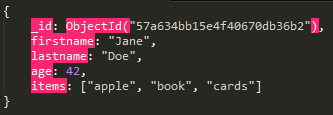
\includegraphics[scale=1]{json_id.PNG}
	
	Figure 2: Data including the 12 byte hexadecimal {\_}id field. In this example the {\_}id was automatically generated from MongoDB. 
\end{center}

\subsection{MySQL}
MySQL is a free open source Relational Database Management System (RDMS) that uses Structured Query Language (SQL) to perform database operations. Unlike MongoDB, MySQL must follow a schema. A schema is a logical group of tables, procedures and views that relate to one type of object (for example an employee schema) (stackoverflow.com, 2017).

MySQL is also fully ACID compliant. ACID stands for: 
\begin{itemize}
	\item Atomic: a transaction that is either fully completed with all of its data modifications or not at all.
	\item Consistent: when the transaction is finished all data must be in a consistent state.
	\item Isolated: modifications to the  data performed by a transaction must be independent of a different transaction.
	\item Durable: when the transaction is completed, effects of the modifications performed by the transaction must be permanent.
\end{itemize}

MongoDB is not as ACID compliant as MySQL. It is compliant at the document level. What MongoDB lacks is transactions. This is the ability to revert any updates to multiple documents (stackoverflow.com, 2017).

Unlike MongoDB, when using MySQL the developer must decide on a primary key to use. This can be any value the developer chooses but a good practice is to use a type of user identifier that is automatically incremented when a new user is entered. The syntax for this statement might look like the following: 

\lstset{frame=tb,
  language=SQL,
  aboveskip=3mm,
  belowskip=3mm,
  showstringspaces=false,
  columns=flexible,
  basicstyle={\small\ttfamily},
  numbers=none,
  numberstyle=\tiny\color{gray},
  keywordstyle=\color{blue},
  commentstyle=\color{dkgreen},
  stringstyle=\color{mauve},
  breaklines=true,
  breakatwhitespace=true,
  tabsize=3
}

\begin{lstlisting}
CREATE TABLE IF NOT EXISTS Users(
	userID INT UNSIGNED NOT NULL AUTO_INCREMENT,
	PRIMARY KEY(userID)
);
\end{lstlisting}

\subsection{ExpressJS}
ExpressJS is a flexible JavaScript web application framework which uses NodeJS to create features for web and mobile applications (expressjs.com, 2017).

It is minimal and provides tools to build applications, with many more plugins available via the Node Package Manager (npm). ExpressJS is similar to Rails for Ruby and Django for Python. Unlike Ruby on Rails or Django there is no documented best way to use the ExpressJS framework. Because it is written in JavaScript and uses NodeJS, express is able to interact with MongoDB in order to retrieve, insert, update and remove documents from a database.

\subsection{AngularJS}
AngularJS is a client-side JavaScript framework that is developed by Google. HTML is useful for declaring static views but fails when trying to declare a dynamic view. Other frameworks deal with this issue by abstracting technologies to manipulate the Document Object Model (DOM). These solutions do not address the root problem which is HTML (angularjs.org/, 2017). AngularJS addresses this issue by extending HTML which is achieved by using directives and binds data to HTML using expressions.

AngularJS is used to develop the frontend elements of a system. Angular uses the Model View Controller (MVC) pattern in order to separate the representations of the data from how it is displayed to the user. Because it is JavaScript based, AngularJS is able to communicate with the other chosen technologies easily.

\subsection{NodeJS}
NodeJS is a server side solution for JavaScript. It is comparable to an Apache webserver for PHP. It is not a JavaScript framework but many of the modules it uses are written in JavaScript. It is built upon Google Cromes V8 JavaScript engine. NodeJS uses an event driven, non-blocking I/O model that makes it lightweight and efficient (nodejs.org/en/, 2017).

A non-blocking I/O (also known as an asynchronous I/O) means that an I/O request will be queued straightaway and the function returns. The I/O is processed at a later point. A blocking I/O thread cannot process anything else until the I/O is complete. In the case of sockets, this could result in a long waiting time. NodeJS uses only one thread to service all requests (stackoverflow.com/, 2017).

The advantage of using NodeJS is that it has its own package manager, similar to Ubuntu, called Node Package Manager (npm for short). This allows developers to share libraries of code as well as managing versions of the code. This is how the ExpressJS framework will be integrated into the project.

\subsection{Apache Server}
The Apache web server is a software product which aims to create a feature rich, robust, commercial grade, open source HTTP server (httpd.apache.org, 2017). 

The features which Apache supports are implemented in compiled modules which can range from server programming to authentication schemes. It is often used with MySQL and PHP to create web applications.

Apache allows developers to control access to different web pages by using different modules that are provided, however it does not give as much control as a NodeJS server. Apache does allow developers to create their own modules however it is not as simple as using NodeJS.

\subsection{Research Conclusions}
From the research completed of the existing games, it is clear that many existing implementations do not address the fact that the difficulty stays the same for the game. The original Space Invaders did have a feature where the enemies would get faster the less there were, however this was a bug that the developer made a mechanic out of. Some solutions to address this problem include creating a template that uses the existing player's data to instantiate a level based on this data. Another solution would be to change properties of the enemy as the game goes on. 

The Unity game engine will be used to implement the functionality of the game. This decision is based on some of the pitfalls of Unreal engine. Although Unreal engine is a more commonly used solution, it did not suit this project. This is because the Blueprints technology used is too simplified and C++ can be over complicated. Unity is a happy medium between these as it uses the C{\#} language for functionality. This also gives the advantage of accessing the .NET framework if necessary. 

For the web application portion of this project MongoDB, ExpressJS, AngularJS and NodeJS technologies will be used. This decision was based on a number of factors. First is previous experience using these technologies. Second is the fact that all these technologies are JavaScript based and MongoDB uses JSON which enables data to be easily passed to and from the server. This is in contrast to using Apache, MySQL and PHP which use different technologies that allow the same functionality. The final factor influencing this decision is that JavaScript technologies are becoming more popular and further experience using these would be beneficial in a future career. 

\newpage
\section{Design}
The design portion of this report will deal with the various thought processes behind the design of the many parts in this project. 

\subsection{Game Design}
Game design is the name given to the various parts of a game. These can include story and plot development, mechanics and aesthetics where applicable. As this game is an arcade game with no story, the design of the game will focus on the mechanics primarily and aesthetics secondly. 

Questions that have to be asked in this section include the following:

\begin{itemize}
\item How does a player play the game?
\item What are the rules of the game?
\item How does the player increase their score?
\item How does the difficulty change as the game is played?
\item What makes the game challenging to the player?
\end{itemize}
Each of these questions will be answered in this section. By the end an in depth knowledge of how the game performs should be acquired. 

\subsubsection{How does the player play the game?}
This project is being developed for the PC platform. Other platforms such as mobile (Android and iOS) were considered but presented some challenges for the outcome. Since a PC is being used, the player will have access to the input hardware that connects to that PC. In layman terms this means the keyboard and mouse. For the purposes of this project, the mouse is only used to click buttons. The player movements are done through the keyboard. 

Before playing the game, the player must create an account on the website. When this is created the player can log into the game and read instructions or begin to play the game. The players spaceship moves left and right by pressing the left arrow key or right arrow key respectively. The A and D keys also provide this functionality for players who prefer using those keys. In order to shoot a laser, the player presses the Space bar. While playing the game, the player can press the Escape key to end the round prematurely if it is required. This will log whatever their recent score is to the database. When the players health becomes 0, the game will log whatever score is accumulated to the database and return to the menu screen.

\subsubsection{What are the rules of the game?}
The rules of this game will follow most of the rules of the original Space Invaders. The player can move left and right until they reach the edge of the screen. From there they will no longer be able to move in the direction they were. When they want to, the player can shoot a laser at the enemy spaceship. These are the only rules that are applicable to this project. Aside from this, players may have their own rules (also known as home brew. For example, players could choose the have a challenge where they can not have a continuous stream of lasers shooting).

One rule that was used in this project is the player's most recent score will be logged. This means that many different players can be on top of the leaderboard.

\subsubsection{How does the player increase their score?}
The player increases their score by successfully shooting and eliminating an enemy spaceship. This will give the player a score increase of 10 points. This differs from the original implementation of Space Invaders where different enemies will give different values depending on their location. Low invaders will give 10 points, middle invaders will give 20 points and upper invaders will score 30 points. There is also a mystery ship that scores between 50 and 300 points.

\subsubsection{How does the difficulty change as the game is played?} 
The game begins easy as all the values to be modified are at their default value. For every 100 points the player scores, one of these values will be randomly chosen and modified and changed. Because it is randomly chosen, the player will not know what values will be modified until it happens.

Another way that the difficulty changes as the game progresses is that the players health never goes up as the game is played. This is in contrast to the original game where for each 1500 points the player scored, they would gain an extra life. This implementation does away with that mechanic as having a set health provides a survival challenge to the player. 

\subsubsection{What makes the game challenging to the player?}
The challenge of this game is achieved by having the enemies randomly increase a value as the player scores more points. As the game progresses, they will become more and more difficult to beat. 

The other challenging part is the fact that only their most recent score will be saved. For example, if on one play through, the player scored 1000 points, it would be saved. If the same player played again and managed to score 0 points, the 1000 points would be overwritten and saved with 0 points.  

\subsection{Database Design}
When discussing database design for a RDBMS there are many different methods to decide which type of data should be stored in a table and how to determine their properties. Such techniques include finding properties such as: 

\begin{itemize}
\item Super keys
\item Candidate keys
\item Primary keys
\item Functionality dependencies
\item Closures
\end{itemize}

With a NoSQL solution such as MongoDB, the same method is not as easily applied. Because of this, decisions had to be made about which types of data should be included. As previously discussed, MongoDB will handle creating unique primary keys which makes the task easier. Because this project has accounts, user names and passwords are required. The possibility that two people will have the same user name is much less than the possibility that they have the same name. 

At a minimum, the database should contain user names and passwords. However, this is not enough information about the user. If something was to go wrong with the account or if the user wanted to delete their account, an email address would be needed. Although this could be achieved with a user name, the user name is public data which could result in other users deleting accounts which they do not own. 

At a minimum, that is the data the must be stored in the database. The next two data fields are used to collect data about how the player plays the game. As such, it is not as critical as the other data fields. Now a schema can be created for this data. As previouly talked about, NoSQL does not strictly enforce this schema so other fields can be added to this. For the purposes of this project however, the schema will be enforced. This is achieved by not allowing the user to input any extra data than is needed. An example of what a document containing user data looks like is as follows:

\begin{verbatim}
{
    "_id" : ObjectId("58d106c002b9ed13e0dc37e3"),
    "email" : "johndoe@gmail.com",
    "username" : "JohnDoe",
    "password" : "mynameisjohndoe",
    "score" : 420,
    "timePlayed" : 13.37
}
\end{verbatim} 

\subsection{Website Design}
The user interface of this website is as minimal as possible. This was decided upon for a number of reasons.
 
\begin{enumerate}
\item It will reduce confusion for new users about where to navigate.
\item Because it will only display some user data and allow account creation, users may opt to use mobile devices to use this website. If there was too much to display, this would increase loading times for users and result in a negative experience. 
\item Companies such as Apple strive for minimal design as it is pleasing to the user and reduces development time for different features (developer.apple.com, 2017).
\end{enumerate}

To achieve this minimal design, the leaderboard should always be displayed as that is the primary use of this website. The data should be displayed in a tabular format which will be pleasing to the user. The only data that will be displayed are the users' user names, their current scores and the total time (in minutes) that they have played. 

The second function of this website is to allow account creation. Because it is secondary, it should only be displayed if the user requests it. This means that there should be a button or text the user clicks to show a form of some sort. Within this form, there should be three text fields to input the data (an email address, a user name and a password). To submit this data there should be a button which submits it. To appeal to the user, the content should be centered where possible.

In order to address the mobile issue, Cascading Style Sheets (CSS) will be used. A framework that puts mobile content first is bootstrap, which will be used in this project (getbootstrap.com/css, 2017). 

\newpage
\section{Implementation}
This section of the report details how the various parts of the project was implemented. It also gives details of some of the problems that came up and how they were solved. It combines the result of the research and design portions of this report. 

\subsection{Game implementation}
From the research completed, C{\#} is being used to program the game. When programming for Unity it can differ from normal C{\#} programming. The following few paragraphs explain how object creation can be achieved in Unity.

This section of the report will explain how objects in Unity can be created, how the game was programmed and how the game interacts with the server to send and receive player information. 

\subsubsection{Unity Object Creation}
In order to interact with Unity specific classes, a class must extend the MonoBehaviour class. This gives the new class access to the Start() and Update() methods. 

The Start() method is executed once, when the class is created. This is generally where objects are initialised and variables are given values where applicable. The Update() method is called once per frame and is where logic that changes is coded. For example, this is where a time value would be incremented.

These are not the only methods that extending the MonoBehaviour class gives access to. Other methods that have been used include: Destroy(), DontDestroyOnLoad(), and Instantiate() to name a few. 

The MonoBehaviour also gave access to some member variables that were used which were the transform variable of type Transform and gameObject variable of type GameObject.  

In order to access the methods from other objects that have extended the MonoBehaviour class it must be done in a different way to normal programming. First, the game object must be found by name. Then the type must be accessed by using the GetComponent() method. Normally the GetComponent() method is a regular method but when interacting with a game object, it has to be a generic method call. An example below is given for what this operation looks like:

\lstset{frame=tb,
  language=Java,
  aboveskip=3mm,
  belowskip=3mm,
  showstringspaces=false,
  columns=flexible,
  basicstyle={\small\ttfamily},
  numbers=none,
  numberstyle=\tiny\color{gray},
  keywordstyle=\color{blue},
  commentstyle=\color{dkgreen},
  stringstyle=\color{mauve},
  breaklines=true,
  breakatwhitespace=true,
  tabsize=3
}

\begin{lstlisting}
public class PlayerContoller : MonoBehaviour
{
	public HealthController h;
	
	void Start()
	{
		h = GameObject.Find("HealthText").GetComponent<HealthContoller>();
		
		//now h can be used like a normal object, for example
		h.setHealth(0);
	}
}
\end{lstlisting}

Not every class has to extend the MonoBehaviour class. As long as the class is not trying to access details specific to unity, objects can be used normally. An example of this in the project is the Player class. It is a helper class used to store information about the player and to save these details when the game is over. To create an object of Player type is achieved as follows: 

\begin{lstlisting}
public class PlayerContoller : MonoBehaviour
{
	private Player p;
	
	void Start()
	{
		p = new Player();
	}
	void Update()
	{
		p.saveDetails("JohnDoe", 420, 13.37);
	}
}
\end{lstlisting}

Now that the details about how object creation and manipulation has been discussed, more details about how the actual game has been programmed can be discussed. The previous paragraphs were required because without understanding how objects are handled, implementing the game would be impossible. 

\subsubsection{Game Programming}
When the game begins all the enemies spawn in. A short animation plays and the spawnTilFull() method is executed. This spawnTilFull() first checks that there is a free position and if there is, a new enemy will be spawned using the Instatiate() method. To continually spawn an enemy, recursion is used that will spawn an enemy with a delay. The code snippet below demonstrates this:

\begin{lstlisting}
		if(freePosition())
		{
			Invoke("spawnTilFull", spawnDelay);
		}
\end{lstlisting}

To check if an enemy should shoot, a simple formula is used. This formula uses the frequency of shooting how long has elapsed since the last frame to determine if a laser should be shot. The formal definition of this formula is: 

\begin{verbatim}
P(shoot) = timeElapsed x frequency
\end{verbatim}

Since this uses Time.deltaTime, it is inserted into the Update() method which is executed once per frame. A random value is then generated using Random.value. If the value generated is less than the probability, the enemy will shoot.  

When an enemy is hit by a laser their health is decreased. If their health reaches zero then the dead() method is executed. This method first adds enemy value to the current score. It then checks if the current score is in the hundreds. If this is true, a value is selected at random. This random value is then used to determine which enemy trait should be modified. The code snippet shows this functionality: 

\begin{lstlisting}
if (scoreController.getScore () % 100 == 0) 
{
	selectedValue = Random.Range (0, numberOfValuesUsed); 

	switch (selectedValue) 
	{
		case 0:
			es.setSpeed (es.getSpeed() + speedModifier);
		break;

		case 1:
			health = health + healthModifier;
		break;

		case 2:
			frequency = frequency + frequencyModifier;
				if (frequency > 0.85) 
				{
					frequency = 0.85f;
				}
		break;
	}
}
\end{lstlisting}

The player functionality is mostly confined to the Update() method in the PlayerController.cs file. This queries the engine to find out if a certain key was pressed and reacts accordingly. To move the player left or right the A, D Left Arrow or Right Arrow key is pressed. These move the player left or right using the following lines of code: 

\begin{lstlisting}
if(Input.GetKey(KeyCode.A) || Input.GetKey(KeyCode.LeftArrow))
{
	transform.position += Vector3.left * speed * Time.deltaTime;
}
else if(Input.GetKey(KeyCode.D) || Input.GetKey(KeyCode.RightArrow))
{
	transform.position += Vector3.right * speed * Time.deltaTime;
}
\end{lstlisting}

The Vector3.left and Vector3.right are a shorthand version of writing Vector3(-1, 0, 0) and Vector3(1, 0, 0) respectively. In the first version of this project, the player would move left and right but the movement wasn't smooth. This was solved by using the speed variable and Time.deltaTime. 

When the Space button is pressed, the InvokeRepeating() method is executed. This takes the name of the method to be executed as a string, the time delay before its executed and the repeat time. When the Space key is released a CancelInvoke() is executed. This works in the same way but it only requires the name of the method. When this was originally programmed there was a bug where only one laser would be shot. This was due to using an else if statement being used instead of an ordinary if statement. 

When the player is hit by an enemy projectile, the OnTriggerEnter2D() method is executed. In this method the players health is decreased. Once the health becomes zero or less the time played is calculated in minutes. This value along with the players name and current score is sent to the server to be updated in the database. After this the game object is destroyed and the scene is destroyed. 

\subsubsection{Game and Server Interaction}
Unity has many options that are available to acquire information form a server. For the purposes of this project the WWW class was used. It is first used in Login.cs in order to connect to the server and use a GET request to download information about the player. This is achieved by firstly getting the player to enter their user name and password. The user name is then added to a string called url which contains the url for the server. In this project, the server is located on localhost. The string is then used to construct the WWW object which gets the player data.

When the player data is successfully acquired it is in JSON format and needs to be parsed. Unity has way of reading and writing JSON which uses a JsonUtility object. When this data is parsed the appropriate variables are assigned and if the password given matches the password that the player has, they are logged in. The following code snippet demonstrates how the JsonUtility is used. 

\begin{lstlisting}
IEnumerator serverInteract(WWW www)
{
	yield return www;

	if(www.error == null)
	{
		string json = www.text;
		p = new Player();
		p = JsonUtility.FromJson<Player>(json);
		uC.setTimePlayed(p.timePlayed);
		uC.setUsername (p.username);
	}
}
\end{lstlisting}

To update the player data proved more troublesome. Since the WWW class was chosen to pass data between the game and server only GET and POST requests were supported. When a POST request was used as a trial it would result in some of the players data being retained and the rest of it would be deleted. This problem was solved by modifying the headers associated with the request. The POST request had to be overridden with a PUT request. The headers variable is of type Dictionary which is a collection of keys and values. In this instance the key and value are of type string. 

The Player object is then converted to JSON which is in turn converted into bytes. This is required to send the data to the server. When all these steps are complete a new WWW object is created but this time has the url, the body (which is a byte array) and the headers.

\begin{lstlisting}
public void saveDetails(string playerName, int playerScore, double playerTime)
{
	json = JsonUtility.ToJson(this);
	body = Encoding.UTF8.GetBytes(json);
	headers.Add("Content-Type", "application/json");
	headers.Add("X-HTTP-Method-Override", "put");
	
	wwwSend = new WWW(url, body, headers);
}
\end{lstlisting}

Even though this way of working proved problematic, it also resulted in an unexpected advantage. Because the Player.cs class doesn't use anything strictly needed by the Unity API, it doesn't need to extend the MonoBehaviour class. This means that all the logic to update the database could be contained in the Player.cs file. 

One problem that was encountered with all this data being passed is that it would be destroyed between scenes. This was solved by using a helper class called UsernameController. 

In this class the Awake() method is called upon. This method is executed before Start() and is used when data needs to be passed between scenes. The singleton design pattern is used here. If there is no instance then the DontDestroyOnLoad() method is called so that when the scene changes, UsernameController still has all the data that it should have. Otherwise the game object is destroyed. 

The UsernameController is used extensively throughout this project where the user data is sent or recieved. The code snippet shows the Singleton design pattern being used. 

\begin{lstlisting}
void Awake()
{
	if (instance == null) 
	{
		DontDestroyOnLoad (gameObject);
		instance = this;
	} 
	else if (instance != null) 
	{
		Destroy(gameObject);
	}
}
\end{lstlisting}

\subsection{Server implementation}
The server used for this project is written in JavaScript by using NodeJS. NodeJS gives users access to many libraries to aid in the development of projects. To get a server running it firstly needs a port number to connect to. It then needs a mechanism to serve data to the user. Initially a middleware platform was not used. This resulted in a few problems relating to Cross Origin Resource Sharing (CORS). After some research it was discovered that the ExpressJS framework should be used as it remedies this problem. 

When the user connects to the url http://localhost:1337 the HTML page for the leaderboard is rendered. The main function for the server is to pass data between the game and server. Some of this data can then be displayed to the user. 

To show the leaderboard to the user a get request is used by ExpressJS, The get request requires a path to obtain the data from and a callback function which specifies whatto to do with the data. The callback has a req variable (short for request) and a res variable (short for response). A database query is then executed using the MongoJS library to find all the entries in the database. If an error occurs (for example, being unable to connect to the database) it is logged to the console. Otherwise the response returns all the documents found in JSON format. 

\begin{lstlisting}
app.get("/userDetails", function(req, res){
    console.log("GET request for /userDetails");

    usersDB.users.find(function (err, docs) {

       if(err)
       {
           console.log(err);
       }
       res.json(docs);
   });
});
\end{lstlisting}

When executing MongoDB queries from a NodeJS server there are many libraries available. MongoDB provide their own library, however this is more tedious than using MongoJS. MongoJS emulates the MongoDB API by wrapping it. The disadvantage to using this library is that not all functionality is emulated by MongoJS but for the purposes of this project it was adequate. 

To insert a new document into the database a post request is used. It is similar to the get request, however the query is different. When a document is inserted it needs data. This is where body property of the request is used. The body contains any information that is relevant to the user. In this case it would be the user name. password, email address, score (which defaults to zero) and the time played (which also defaults to zero). 

\begin{lstlisting}
usersDB.users.insert(req.body, function(err, doc){
	if(err)
	{
		console.log(err);
	}
	res.json(doc);
});
\end{lstlisting}

In order for the user to log in from the game, another get request is used. This time the path is altered. It now uses route parameters to find a user which matches the user name given given.

A new variable called query is then created which is written in JSON format. This variable is then used in a MongoDB query to find the matching record. If MongoDB was unable to locate the user then an error is logged, other wise the user data is returned. 

\begin{lstlisting}
app.get("/userDetails/:username", function(req, res){
    var username = req.params.username;
    var password = req.params.password;

   console.log("Recieved a GET request for " + username);

   var query = {
                    "username": username
                    //"password": password
               };

    usersDB.users.findOne(query, function(err, docs){
      if(err)
      {
          console.log(err);
      }
        res.json(docs);
   });
});
\end{lstlisting}

In the example shown above the user name and password are extracted from the request using the req.params.username and req.params.password properties.

When a user plays the game, their most recent score is kept and their total time played is updated. To get this functionality, a put request is normally used. However as previously explained in section 4.1.3 Game and Server Interaction, this proved troublesome. The game had to override the post method and the server has to accept this. This was achieved by the server accepting a x-www-form-urlencoded. Another solution to this would be to use multipart/form-data however it is recommended to only use a multipart/form-data when sending large amounts of binary data or non ASCII characters (www.w3.org, 2017). Because all the data to be passed to the server uses ASCII characters, the x-www-form-urlencoded was deemed acceptable. 

Although the server uses the post command to accept the incoming data, in this instance it mimics a put command. This allows the data to be updated easily. 

\begin{lstlisting}
app.post("/userDetails/:username", function(req, res){
    console.log("Updataing details for " + req.body.username);
    console.log("SCORE: " + req.body.score + ", TIME: " +req.body.timePlayed);

    usersDB.users.findAndModify({
        query: { username: req.body.username },
        update: { $set: {score: req.body.score, timePlayed: req.body.timePlayed}},
        new: true }, function(err, doc) {
        if(err) { console.log("Error " + err); }
        res.json(doc);
    });
});
\end{lstlisting}

There was a problem here when the server was originally implemented. When accessing the username, score and timePlayed variables, req.params was used. However after some debugging it was realised that the req.body property was the correct way to access the data. When the data was successfully acquired, a query could now be written. 

THe findAndModify operation uses a query parameter which is a document (in this case it is the username). Then the update parameter is then executed which requires an update operator which is the {\$}set operator in this case. Following this is the new parameter which returns the updated document when set to true. 

When updating doecuments, there are many operations that can be used, for example the update operation could have been used here too. The reason why it was not used is because the update operation is more suited for updating multiple documents rather than one. 

\subsection{Webpage implementation}
The web page for this project uses HTML, CSS and the Angular MVC Framework to pass data to the server. To get Angular to work, the Angular JavaScript file must be linked to the HTML page. This can be done in two ways. It can either be included using the URL to the file or by firstly downloading the JavaScript file and including it in a script tag. The code snippet shows both or these methods. 

\begin{lstlisting}
<!--method one-->
<script src="https://ajax.googleapis.com/ajax/libs/angularjs/1.4.8/angular.min.js">
</script>

<!--method two-->
<script src="js/angular.min.js"></script>
\end{lstlisting}

A decision was made early in the development to use the second method. This has the advantage of not relying on connecting to the URL that connects to the file every time the script is required. For example if there was a network error which resulted in not being able to connect to the URL then none of the Angular functionality would work.

The ng-app directive is used to designate the root of the web page. It is generally set near the beginning of the web page. The ng-controller directive sets a controller class for the view. This allows data to be passed between the client (the web page) and the server. 

Once the controller is set in HTML, the logic can be programmed using JavaScript. This can be included in the HTML file using the <script> tag or in a seperate JavaScript file. For this project a seperate JavaScript file is used. In the JavaScript file the module must first be registered using the angular.module() function. When this is done, the controllers can be programmed. 

When using angular it is advised to keep controllers as small as possible. This project has two controllers, the LeaderboardController and the CreateAccountController. The LeaderboardController gets all the user data from the server, adds it to a user object (which is the model) and then passes it to the HTML page (which is the view). This controller also handles users deleting their accounts. To achieve this the user must use their email address. The {\$}http service then sends a delete request to the server if the email address matches the one associated with the account. The page is then reloaded which will result in the leader board being updated.  

\begin{lstlisting}
app.controller("LeaderboardController", ["$scope", "$http", function($scope, $http) {

    $scope.user = [];

    function getDetails()
    {
        $http.get("/userDetails").success(function(res){
            $scope.user = res;

        });
    };

    getDetails();


    $scope.remove = function(id, email){
        console.log(id);
        console.log(email)

        var inputEmail = prompt("Please enter the email address associated with this account to remove it")

        if(inputEmail.toLowerCase() === email)
        {
            $http.delete("/userDetails/" + id).success(function(responce){
                alert("You were successfully removed. Page will now reload.");
                location.reload();
            });
        }
        else
        {
            alert("Error, wrong email inputted. Don't try to delete other peoples accounts");
        }
    };
}]);
\end{lstlisting}

The leader board will only display the top five users with the highest score. To get this functionality working a filter is used on the HTML page. Filters work by returning a new array which contains the subset of items required.

\lstset{frame=tb,
  language=html,
  aboveskip=3mm,
  belowskip=3mm,
  showstringspaces=false,
  columns=flexible,
  basicstyle={\small\ttfamily},
  numbers=none,
  numberstyle=\tiny\color{gray},
  keywordstyle=\color{blue},
  commentstyle=\color{dkgreen},
  stringstyle=\color{mauve},
  breaklines=true,
  breakatwhitespace=true,
  tabsize=3
}

\begin{lstlisting}
<tr ng-repeat="u in user | orderBy: '-score' | limitTo: 5 " align="center">
	<td>{{u.username}}</td>
	<td>{{u.score}}</td>
	<td>{{u.timePlayed}}</td>
	<td><button class="btn btn-danger btn-xs" ng-click="remove(u._id, 						u.email)">Remove</button></td>
</tr>
\end{lstlisting}

In this example the filter takes all the users, orders them by score in descending order and only shows the top 5 users. The ng-repeat directive is similar to a forEach loop. It loops over all the users and displays the properties that are required. The ng-click directive allows a user to be deleted by giving the name of the function and the arguments to be passed to the function. The logic is handled in the JavaScript file as previously seen. 

The second controller that is used is the CreateAccountController. This controller gathers all the user data that is inputted, sets the score and time played to the default values (zero) and posts them to the server. When this is successfully executed the page is refreshed however if there are more than five users in the table, they new user will not be shown. 

The CreateAccountController has a toggle function. This is used by the ng-click directive to show the user creation form. The {\$}scope object is what enables data to pass between the contoller and view. In the toggle function it is setting the value of createAccount to be inverted. (i.e if it is true, it will set it to false). This is used by the ng-show directive to display the form.

When dealing with user input one problem that arises is form validation. Angular handles this problem by having many different directives that can assist in validating information. This is evident in form where it specifies what the mimimum length for the password and user name fields must be. For the user to be able to create an account all the data entered must meet a certain criteria (password must have a minimum length, email address must be in a valid format and no field can be empty). Normally this would be a difficult task however the ng-disabled directive takes care of this. If any of the fields are invalid, the button to submit the data can not be clicked. When everything is valid, the button can be clicked and the user will have an account. 

\lstset{frame=tb,
  language=html,
  aboveskip=3mm,
  belowskip=3mm,
  showstringspaces=false,
  columns=flexible,
  basicstyle={\small\ttfamily},
  numbers=none,
  numberstyle=\tiny\color{gray},
  keywordstyle=\color{blue},
  commentstyle=\color{dkgreen},
  stringstyle=\color{mauve},
  breaklines=true,
  breakatwhitespace=true,
  tabsize=3
}

\begin{lstlisting}
<div><a href="" ng-click="toggle()">Don't have an account? Create one here!</a>
</div>
<br>

<div ng-show="createAccount">
	<input name="email" type="email" class="form-control" placeholder="Email" ng-model="user.email" required>
	<br>
	<input name="username" type="text" class="form-control" placeholder="Username (minimum 4 characters)" ng-model="user.username" ng-minlength="5" required>
	<br>
	<input name="password" type="password" class="form-control" placeholder="Password (minimum 8 characters)" ng-model="user.password" ng-minlength="8" required>
	<br>
	<button type="button" class="btn btn-primary" ng-disabled="form.email.$invalid || form.password.$invalid || form.username.$invalid" ng-click="createUser()">Create Account</button>
	<br><br><br>

	<div class="alert alert-info">
		<p><b>Suggestion: </b> use a different password than your usual one.</p>
		</div>
</div>
\end{lstlisting}

\newpage
\section{Testing and Evaluation}
In this section the testing and evaluation of the project will be discussed. This will go through how the game was tested and how the website was tested. During the development of this project I developed a bug reporting web page. 

This page was used during demo day to keep track of any issues that users encountered for any part of the project. This web page collected the users information about the issue and sent it to the server. When this information reached the server it was entered into another collection in MongoDB (called bugs) and also outputted to a file called bugs.json. The bugs.json file is included in Appendix 1 of this report. 

\subsection{Game Testing}
While developing the game it was continually tested however this was done by myself. While this was a good strategy for finding small problems (such as the shooting problem mentioned is section 4.1.2 Game Programming). To remedy this, some independent testing from outside users was required. The project Demo Days provided this. Many people were able to play the game and provide feedback. 

One problem that was found was that users with a space in their user name could create an account but could not log in (for example John Doe).

Another bug that was found was that often it was possible to kill enemies before they finished spawning in. This lead to users getting increasing scores without properly playing the game. However the game managed to fix this itself because the enemies could also shoot at the player as they were spawning. 

Another example of a problem and perhaps the one that annoyed users the most was that when their health was decreased to zero the game would not send the new score to the server. Originally I thought this would be an interesting challenge however it was noted that it was annoying for the users. I took this information into consideration and programmed the game to update the score when the user quits or when their health becomes zero.

\subsection{Server Testing}
Because the server is an integral part of this project it needed to be tested. Testing a server that uses NodeJS is simplified because many testing frameworks are freely available through the Node Package Manager (npm). The testing framework chosen for this project is Mocha. Mocha was chosen because it supports many different types of testing paradigms such as Behaviour Driven Development (BDD) and Test Driven Development (TDD). The testing paradigm used in this project is Behaviour Driven Development. 

To use Mocha, first a new directory must be created where all test cases will reside. In the package.json file (which contains data about the server), the test script must be set up to link to mocha by inputting mocha beside the test key. The package.json file is available in Appendix 2. When these steps are completed, test cases can be written and can be run using the npm test command. 

\lstset{frame=tb,
  language=csh,
  aboveskip=3mm,
  belowskip=3mm,
  showstringspaces=false,
  columns=flexible,
  basicstyle={\small\ttfamily},
  numbers=none,
  numberstyle=\tiny\color{gray},
  keywordstyle=\color{blue},
  commentstyle=\color{dkgreen},
  stringstyle=\color{mauve},
  breaklines=true,
  breakatwhitespace=true,
  tabsize=3
}

The first test case in this project tests if the homepage is available. If it does, the status code will return 200 which means it exists. 

\begin{lstlisting}
describe("/", function(){
    it("homepage should return 200", function(done){
        http.get("http://localhost:1337", function(res){
            assert.equal(200, res.statusCode);
            done();
        });
    });
});
\end{lstlisting}

The second test case checks if the userDetails parameter is available. Like the first case, if it is the status returned will be 200.

\begin{lstlisting}
describe("/userDetails", function(){
    it("homepage should return 200", function(done){
        http.get("http://localhost:1337", function(res){
            assert.equal(200, res.statusCode);
            done();
        });
    });
});
\end{lstlisting}

The third test case that runs tests if the users information can be reached and returns status 200 if it can be reached.

\begin{lstlisting}
describe("/userDetails/RianF2", function(){
    it("homepage should return 200", function(done){
        http.get("http://localhost:1337", function(res){
            assert.equal(200, res.statusCode);
            done();
        });
    });
});
\end{lstlisting}

The fourth test case is different. Firstly it checks if a user that doesn't exist can be reached. Secondly it checks what data is associated with that user. From experimentation it was revealed that null should be returned if a non existent user is requested. However the first test case will return status 200. The second test case will fail. This is a problem for which a solution has still not been found. 

\begin{lstlisting}
describe("/userDetails/kanye", function(){
    it("/userDetails/kanye should return 200", function(done){
        http.get("http://localhost:1337/userDetails/kanye", function(res){
            assert.equal(200, res.statusCode);
            done();
        });
    });

    it("but should return null when kanye is requested", function(done){
        http.get("http://localhost:1337/userDetails/kanye", function(res){
            var data;

            res.on("data", function(chunk){
               data += chunk;
            });

            res.on("end", function(){
                assert.equal(null, data);
                done();
            });
        });
    });
});
\end{lstlisting}

Appendix 3 contains an image from what the test cases look like when they are run.

\newpage
\section{Conclusions and Further Development}
Overall the project was a success. It achieved what it was supposed to which was:

\begin{itemize}
\item Improve the classic game of Space Invaders by making the game harder to beat the higher score the user achieves.
\item I became familiar with the Unity engine and can now use it to create games.
\item I was able to increase my knowledge of web based technology.
\item I was able to apply much of what I have learned throughout my course.
\end{itemize} 

If this project was to be developed further there are a number of things that would be done differently. 

Firstly when the game interacts with the server, a UnityWebRequest would be used over the WWW class. This is because the UnityWebRequest class allows the HTTP PUT method to be used. This would mean that the headers would not need to be overridden  when the game updates the user details.

Secondly, when testing the server more consideration would be put into what frameworks should be used and how test cases should be written. Mocha was chosen simply because it was the first result that a Google search returned. This was a bad decision because the advantages and disadvantages of Mocha were not taken into consideration. Part of this decision was also due to running out of time before the project was due to be submitted. 

One last thing that I would develop further is how passwords are handled. In its current state the project does not encrypt passwords. This is a major security flaw which is not acceptable in applications that handle user data. 

\newpage
\section*{References}
\addcontentsline{toc}{section}{\protect\numberline{}References}

Angularjs.org (2017) \textit{ngController} [online], available: https://docs.angularjs.org/api/
\hangindent=0.5in ng/directive/ngController [accessed 1 January 2017]

Apache (2017) \textit{What is the Apache HTTP Server Project?} [online], available: https://
\hangindent=0.5in httpd.apache.org/ABOUT{\_}APACHE.html{\#}What [accessed 6 April 2017]

Atari 2600 Specifications (2016) \textit{Technical Data} [online], available: http://problemka
\hangindent=0.5in putt.de/2k6specs.htm [accessed 29 December 2016]

Apple (2017) \textit{iOS Human Interface Guidelines} [online], available: https://developer.a
\hangindent=0.5in pple.com/ios/human-interface-guidelines/visual-design/layout/ [accessed 11 A
\hangindent=0.5inpril 2017]

Bandai Namco \textit{Space Invaders Evolution} [online], available:
https://www.bandainam
\hangindent=0.5incinoent.eu/product/space-invaders-evolution/psp [accessed
4 January 2017]

Bootstrap \textit{Overview} [online], available: http://getbootstrap.com/css/ [accessed 11 \hangindent=0.5in April 2017]

Express (2017) \textit{Web Application} [online], available: http://expressjs.com/ [accessed 
\hangindent=0.5in 1 January 2017]

Gamespy (2016) \textit{The Gamespy Hall of Fame} [online], available: https://web.archive.
\hangindent=0.5in org/web/20080408152913/http://archive.gamespy.com/legacy/halloffame/spa
\hangindent=0.5inceinvaders.shtm [accessed 30 December 2016]

IGN (2008) \textit{Space Invaders Extreme} [online], available: http://ie.ign.com/games/spac \hangindent=0.5ine-invaders-extreme/nds-965078 [accessed 4 January 2017]

JSON (2017) \textit{Introducing JSON ECMA-404 The JSON Data Interchange Standard} [online], available: \hangindent=0.5in http://www.json.org/ [accessed 1 January 2017]

Kotaku (2016) \textit{Space Invaders Infinity Gene Micro-Review: Evolve or Die} [online], 
\hangindent=0.5in available: http://kotaku.com/5328750/space-invaders-infinity-gene-micro-rev
\hangindent=0.5in iew-evolve-or-die [accessed 30 December 2016]

MongoDB (2017) \textit{BSON Types} [online], available: https://docs.mongodb.com/manua
\hangindent=0.5in l/reference/bson-types/{\#}objectid [accessed 1 January 2017]

NodeJS (2017) \textit{Home} [online], available: https://nodejs.org/en/ [accessed 2 January 
\hangindent=0.5in 2017]

Stack Overflow (2009) \textit{What good are SQL Server schemas?}, [online] available: http://
\hangindent=0.5in stackoverflow.com/questions/529142/what-good-are-sql-server-schemas [acces
\hangindent=0.5in sed 5 April 2017]

Stack Overflow (2017) \textit{MongoDB} [online], available:
http://stackoverflow.com/questi
\hangindent=0.5inons/tagged/mongodb [accessed 1 January 2017]

Stack Overflow (2011) \textit{What does MongoDB not being ACID compliant really mean?} \hangindent=0.5in[online], available: http://stackoverflow.com/questions/7149890/what-does-m
\hangindent=0.5in ongodb-not-being-acid-compliant-really-mean [accessed 5 April 2017]

Stack Overflow (2013) \textit{What is non-blocking or asynchronous I/O in Node.js?} [on
\hangindent=0.5in line], available: http://stackoverflow.com/questions/10570246/what-is-non-bl 
\hangindent=0.5inocking-or-asynchronous-i-o-in-node-js [accessed 2 January 2017]

The International Arcade Museum (2016) \textit{Space Invaders} [online], available: http://w
\hangindent=0.5in ww.arcade-museum.com/game{\_}detail.php?game{\_}id=9662 [accessed 29 December 2016]

The ISO Zone (2015) \textit{Space Invaders} [online], available:
http://www.theisozone.com/
\hangindent=0.5in downloads/pc/windows-games/space-invaders-12/
[accessed 4 January 2017]

Unity (2016) \textit{Build once, deploy anywhere} [online], available: https://unity3d.com/un
\hangindent=0.5in ity/multiplatform [accessed 30 December 2016]

Unity (2009) \textit{How should I decide if I should use C{\#}, JavaScript (UnityScript) or 
\hangindent=0.5in Boo for my project?} [online], available: http://answers.unity3d.com/questions/75
\hangindent=0.5in 28/how-should-i-decide-if-i-should-use-c-javascript-u.html [accessed 30 December 2016]

Unity (2015) \textit{Will Boo ever come back?} [online], available:
https://forum.unity3d.com
\hangindent=0.5in m/threads/will-boo-ever-come-back.375988/ [accessed 30
December 2016]

Unreal (2014) \textit{[Twitch] Fortnite Developers Discussion - Apr. 17, 2014} [online], \hangindent=0.5in available: https://forums.unrealengine.com/showthread.php?3035-New-Twitch--w
\hangindent=0.5inith-Fortnite-developers-Thursday-April-17{\&}p=19464
\hangindent=0.5in{\&}viewfull=1{\#}post19464 [accessed 05 April 2017]

Unreal (2017) \textit{What is Unreal Engine 4} [online], available: https://www.unrealengine
\hangindent=0.5in .com/what-is-unreal-engine-4 [accessed 5 April 2017]

W3C Reccommendation (2017) \textit{17 Forms} [online], available: https://www.w3.org/TR
\hangindent=0.5in/html401/interact/forms.html{\#}h-17.13.4.1 [accessed 5 April 2017]

\newpage
\section*{Appendices}
\addcontentsline{toc}{section}{\protect\numberline{}Appendix}
\textbf{Appendix 1:} The bugs.json file showing bugs found during demo day

\textbf{Appendix 2:} The package.json file showing information about the server

\textbf{Appendix 3:} The result of tests being run on the server
\newpage
\textbf{Appendix 1:} The bugs.json file
\begin{lstlisting}

\end{lstlisting}
\textbf{Appendix 2:} The package.json file
\begin{lstlisting}
{
  "name": "website",
  "version": "1.0.0",
  "description": "the website/server portion of fyp",
  "main": "server.js",
  "dependencies": {
    "body-parser": "^1.16.0",
    "express": "^4.14.0",
    "mongojs": "^2.4.0",
    "node-gyp": "^3.5.0"
  },
  "devDependencies": {},
  "scripts": {
    "test": "mocha",
    "start": "node server.js"
  },
  "keywords": [
    "final",
    "year",
    "project"
  ],
  "author": "Rian Fitzgerald",
  "license": "MIT"
}
\end{lstlisting}

\newpage
\textbf{Appendix 3:} The output from the test cases being run

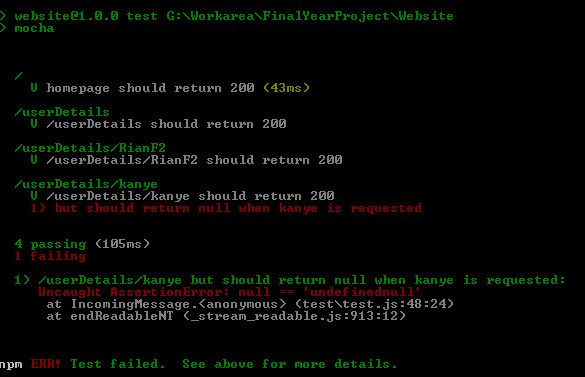
\includegraphics[scale=1]{test.png}

\end{document}